Although there have been uncertainties in capturing the topography of the ocean near shore, mathematical methods can estimate bathymetry using the dispersion relationship between wavelength and the period. Stockdon et al. used video imagery, which compared true wave signal and remotely sensed video signal to create a linear representation between wave amplitudes and phases \citep{stockdon2000}.  Holman et al. used a 2-dimensional method with Kalman filtering to estimate the depth, $h$ \citep{holman2013}.

We invert for depth, \textit{h}, using wave length and wave number with a 1D model derived using the energy flux method to create a correlation between wave length and depth from the water surface as shown in Figure~\ref{flowchart}.

\begin{figure}[h]
		\centering
		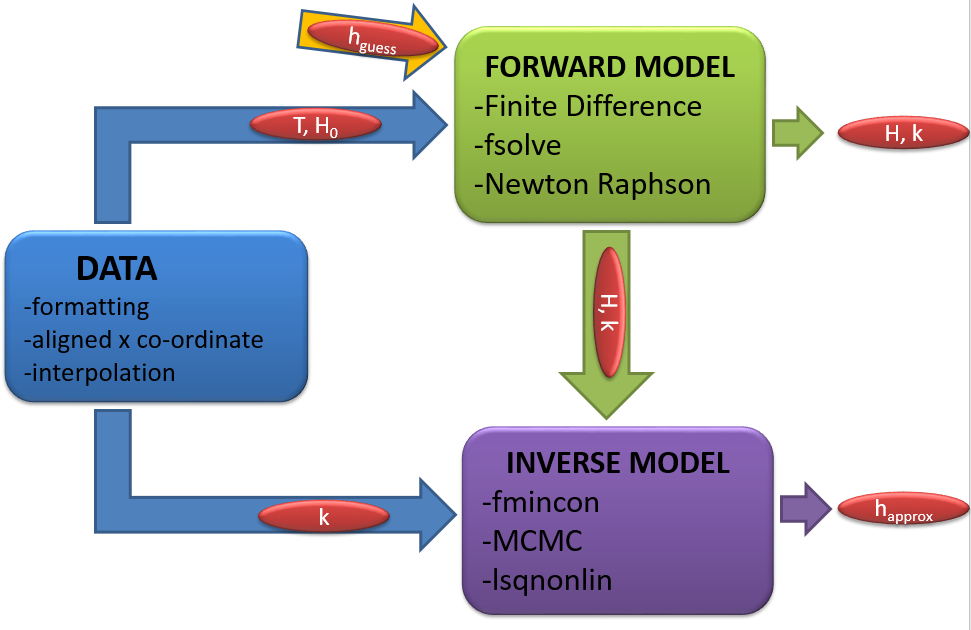
\includegraphics[width=.6\linewidth]{img/Flow_Chart.png}
		\caption{Flow chart of the workflow for this research}
		\label{AWAC}
\end{figure}

\subsection{Forward Problem}\label{forwardproblem}
The forward problem is described by 1D linear wave theory:
\begin{eqnarray}
\label{fp1}
\left \{
\begin{array}{lll}
\frac{d}{dx}\left(EC_g\right)=-\delta,\\
\\
\sigma^2=gk\tanh(kh),
\label{ode}
\end{array}
\right.
\end{eqnarray}
where $\delta$ is  wave breaking parameter and the speed at which the energy is transmitted, $C_g$, called linear theory group speed, is given as
\begin{equation}
\label{cg}
C_g=\frac{c}{2}\left(1+\frac{2kh}{\sinh(2kh)}\right),
\end{equation}
with $c=\frac{\sigma}{k}$ and from the linear theory, the wave energy, $E$ is given as
\begin{equation}
\label{e}
E=\frac{1}{8}\rho g H_{rms}^2,
\end{equation}
$\rho$ is the density of water, $g$ is the gravitational acceleration, $\sigma$ is the angular frequency, $c$ is the local wave phase speed, $k$ is the wave number, $h$ is the water depth and $H$ is the wave height. Here, we assume $T$, the wave period, is constant.\\ 

\noindent Observe that equation \ref{fp1} is coupled using the fact that $\sigma=\frac{2\pi}{T}$. Hence, using equation \ref{cg} and \ref{e} in \ref{fp1}, we obtain
\begin{equation}
\label{fpdelta}
\frac{d}{dx}\left( \frac{\lambda}{k}\left(1+\frac{2kh}{\sinh(2kh)}\right)H^2 \right)=-\delta,
\end{equation}  
and 
\begin{equation}
\label{fk}
f(k) = gk\tanh(kh)-\sigma^2,
\end{equation}
where $k$ is the zero of function $f$ and $\lambda=\frac{\rho g \pi}{8T}$.\\

The wave breaking function, $\delta$, proposed by (Janssen and Battjes, 2007) is given as
\begin{equation}
\delta = \frac{1}{4h}B\rho g f H_{rms}^3\left[(R^3+\frac{3}{2}R)exp(-R^2)+\frac{3}{4}\sqrt{\pi}(1-erf(R))\right],
\end{equation}
This breaking function is basically depends on the wave height ${H}$ using the following parameters in terms of ${H}$\\
$$R=\frac{H_b}{H_{rms}}, \quad H_{rms} = 0.7H,\quad H_b=0.78h,\quad f=\frac{1}{T},\quad B=1.$$
In the above expression ${H_{b}}$ is the local wave breaking height, ${H_{rms}}$ is the root mean square of height and ${f}$ represents frequency. We can see that ${R}$ is wave breaking condition is provided 

\subsection{Numerical Solution of the Forward Model}
A finite difference scheme is applied to obtain a numerical solution with appropriate initial and boundary conditions. In the scheme of finite differences, the derivatives are replaced using their finite-difference approximations. The goal is to provide wave height using the finite difference method. In the process, MATLAB's fsolve function is applied to obtain the wave number. Furthermore, the Newton-Raphson method is used to verify the solution of wave number $k$ obtained by the fsolve function.
\subsubsection{Discretization of the Model}
A forward difference method is applied depending on the nature of the model given in equation (\ref{fpdelta}). The main goal is to obtain the wave height${H}$. In the process we calculate the following terms:\\
Total energy per unit area
$${E=\frac{1}{8}\rho g H_{rms}^2}$$\\
where ${\rho}$ is water density 1000${kg/m^3}$ and ${g}$ represents the gravitational acceleration ${9.8m/sec^2}$. \\
The root mean square of height as\\
$${H_{rms}=0.7 H}$$\\
Group wave celerity will be defined as in  (\ref{cg}). The wave period is provided from the original data with boundary condition ${H_{0}}$. 
Wave number plays an important role in estimating the wave height as well. To calculate the wave number MATLAB function fsolve used as non-linear solver to find the zeros of the function given in (\ref{fk}) obtained from the dispersion relationship
$$
\sigma^{2}=gk tanh(kh).
$$ 
So, at each index point, wave number, $k$, is generated with initial guess $k_0$:
$$k_0=\frac{\sigma}{\sqrt{gh}}.$$
This initial condition is chosen because in shallow water the dispersion relation provides \\
%$${c=\frac{\sigma}{k}\simeq\sqrt{gh}}
$${\sigma^2\simeq g\,k^2\,h}$$

Newton-Raphson method is applied to verify the wave number from fsolve. Therefore, using same initial condition the approximate solution is obtained from
\begin{eqnarray}
k_{i+1}& =& k_{i}-\frac{gk_i\tanh(k_ih)-\sigma^2}{g\tanh(k_ih)-ghk_i sech^2(k_ih)},
\end{eqnarray}

Thus at each index forward finite difference expression is calculated as
$$E_{i}=\frac{\delta_{i-1}\Delta x}{(C_g)_{i}}+\frac{E_{i-1}(C_g)_{i-1}}{(C_g)_{i}}$$
In the above expression ${\Delta x}$ represents the mesh spacing. We have applied equal spacing for this numerical scheme.After estimating the energy ${E}$ at each index points we update the value of the root mean square of height ${H_{rms}}$. This updated value is applied in the ${H=\frac{H_{rms}}{0.7}}$ to obtain the wave height at each index points. 


%\begin{comment}
%A forward difference method is applied depending on the nature of the model given in equation (\ref{fpdelta}).\\
%Let 
%$$c^{*} = \frac{c_{g}\lambda}{k},\quad c_{g} = nc =\frac{2\pi n}{T},$$
%with 
%$$\lambda = \frac{1}{8}\rho g, \quad n = \frac{1}{2}\left(1+\frac{2hk}{sinh(2hk)}\right).$$
%Let $\widetilde{H}=H^{2}$. Then the ordinary differential equation of the model given in (\ref{fpdelta}) becomes
%\begin{equation}
%\frac{d}{dx}\left( c^{*}\widetilde{H}\right)=-\delta
%\end{equation}
%Applying the finite difference method, the above expression becomes
%$$
%\frac{c_{i}^{*}\widetilde{H}_{i}-c_{i-1}^{*}\tilde{H}_{i-1}}{\triangle x}= \delta \quad \Rightarrow \quad
%\widetilde{H}_{i}=\frac{c_{i-1}^{*}\widetilde{H}_{i-1}+\triangle x \delta}{c_{i}^{*}}
%$$
%Hence, at each index point in the discretization, $
%H=\sqrt{\widetilde{H}}$.
%\subsubsection*{MATLAB function fsolve}
%As part of the process of obtaining wave height, $H$, MATLAB function fsolve is used as non-linear solver to find the zeros of the function given in (\ref{fk}) obtained from the dispersion relationship
%$$
%\sigma^{2}=gk tanh(kh).
%$$ 
%So, at each index point, wave number, $k$, is generated with initial guess $k_0$:
%$$k_0=\frac{\sigma}{\sqrt{gh}}.$$
%\subsubsection*{Newton-Raphson Method}
%The Newton-Raphson method is a widely used method for finding roots. This method is used in the numerical experiment to verify the wave number extracted using MATLAB function fsolve. Therefore, approximate solution using Newton-Raphson method is obtained as
%\begin{eqnarray}
%k_{i+1}& =& k_{i}-\frac{gk_i\tanh(k_ih)-\sigma^2}{g\tanh(k_ih)-ghk_i sech^2(k_ih)},
%\end{eqnarray}
%using the same initial guess as for fsolve.
%This provides the wave number, $k$, for each index.
%\end{comment}
\subsubsection{Implementation}
To apply the finite difference method we first discretize the space vector, ${x}$, depending on predefined mesh size, ${\Delta x}$. For the numerical experiments we usually applied $\Delta x=10$ and ${\Delta x=25}$ which means index points are set in ${10m}$ and ${25m}$ apart respectively. Wave breaking condition is supplied using the breaking parameter ${\delta}$.
%The wave breaking condition applied in this experiment is
%$${H=0.78h}$$
%The reason for this condition is the model is focused on the shallow water. In shallow water the individual wave breaks when the wave height  ${(H)}$ and depth ${h}$ relationship is 
%$${H>0.8h}$$

The implementation of the algorithm is as follows
\begin{algorithm}
\caption{Algorithm to estimate wave height H}\label{euclid}
\begin{algorithmic}[1]
\Procedure{}{}
\BState \emph{\textit{\textbf{Initialization}}}:
\State $\textit{Mesh spacing:\,\,} \Delta x$

\State $\textit{Initial depth:\,\,} h$
\State $\textit{Wave period:\,\,} T$
\State $\textit{Boundray condition of height:\,\,}H_{0}$
\BState \emph{\textbf{Step 1: Estimate wave number k}}
\State $\bullet \quad\sigma=\frac{2\, \pi}{T}$

\State $\bullet \quad\sigma^2=gk\tanh(kh)$

%\State $\textit{Wave breaking:\,\,}\delta$
%
%\BState \emph{\textbf{Step 1:}}
%\State $\bullet \quad\textit{constant}\quad \lambda=\frac{ \rho g \pi}{8T}$
%
%\BState \emph{\textbf{Step 2:}}
%\State $\bullet \quad\textit{Find\,\,} c^{*} \textit{\,\,depending on \,\,}k:\quad c^{*}=\frac{(1+(2kh)}{sinh(2kh)}\lambda \,\, k$

\BState \emph{\textbf{Step 3:Compute wave height H}}
\State $\bullet \quad\textit{Compute wave breaking function:\,\,} \delta$
\State $\bullet \quad\textit{Compute wave group celerity:\,\,} C_g$
\State $\bullet \quad\textit{Compute:\,\,} H:\quad E_{i}=\frac{\delta{i-1}*\Delta x}{(C_g)_{i}}+\frac{E_{i-1}*(C_g)_{i-1}}{(C_g)_{i}}$
\State $\bullet \quad\textit{Update :\,\,} (H_{rms})_{i}=\sqrt{\frac{8.0\,E_{i}}{\rho\, g}}$
\State $\bullet \quad\textit{Compute :\,\,} H_{i}=\frac{(H_{rms})_{i}}{0.707}$
\EndProcedure
\end{algorithmic}
\end{algorithm} 


\subsubsection{Numerical Results}
We present some of the numerical results in the following Figures.

%%%%%%%%%%%%%%%%%%%%%%%%%%%%%%%%%%%%%%%%%%%%%%%%%%%%%%%%%

\begin{figure}[h]
\begin{minipage}[b]{0.47\linewidth}
\centering
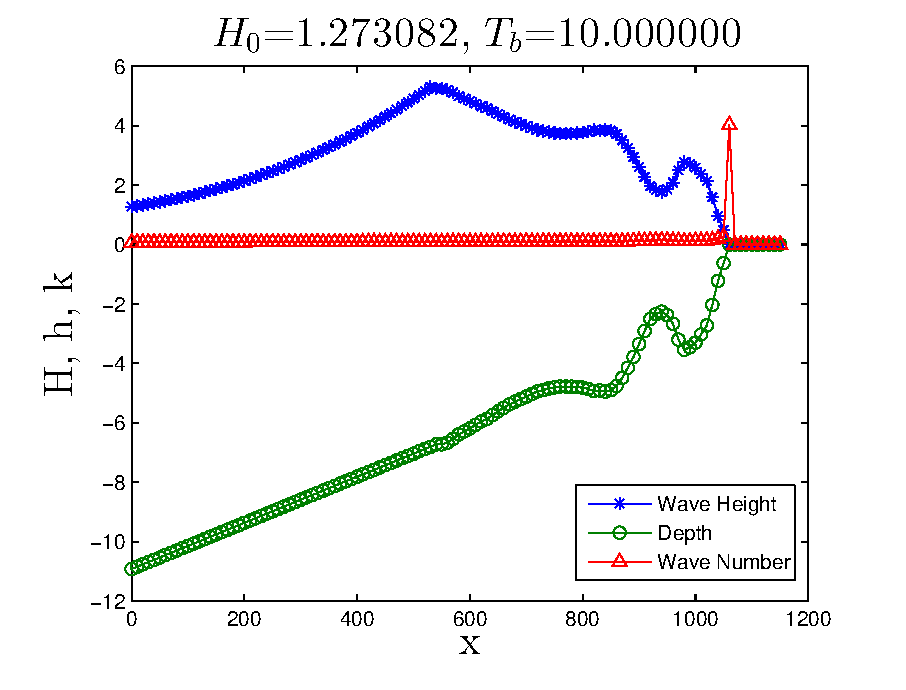
\includegraphics[width=\textwidth]{forward_plot/p1_1.eps}
%\caption{Case I: Water Depth(h), Wave Height(H) and Wave Number vary with x direction}
\label{FigHhk_1}
\end{minipage}
\hspace{0.2cm}
\begin{minipage}[b]{0.47\linewidth}
\centering
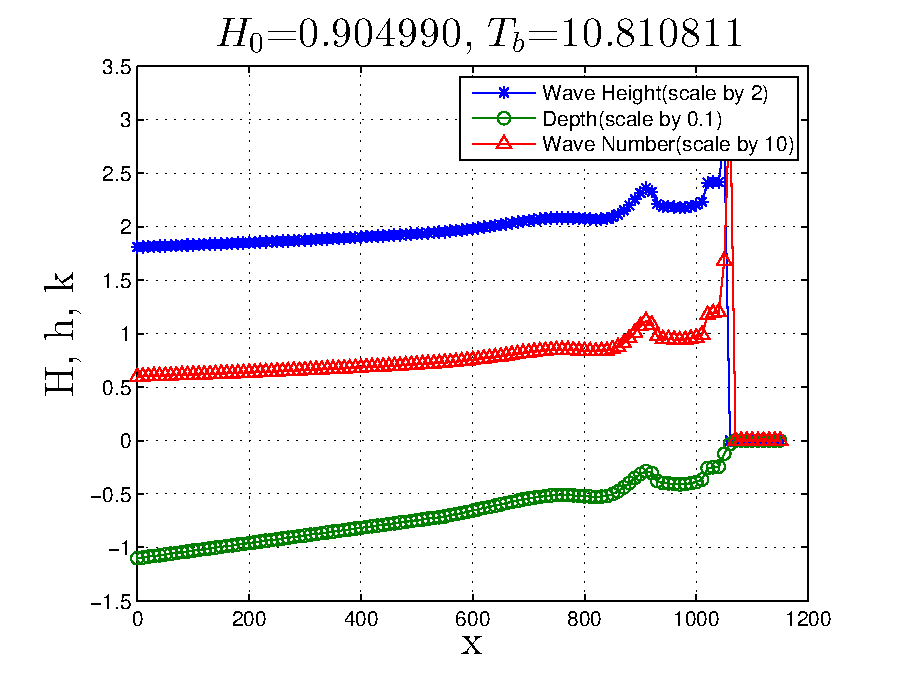
\includegraphics[width=\textwidth]{forward_plot/p2_1.eps}
%\caption{Case II: $N=500$}
\label{FigHhk_2}
\end{minipage}
\caption{Water Depth(h), Wave Height(H) and Wave Number vary along x direction (Two sets of boundary conditions are applied for following figures. The boundary conditions for the left is extracted from the data of 2015/10/9 22:00-23:00 and for the right is extracted from the data of 2015/10/9 03:00-04:00). Note that $x=0 m$ is located offshore at the boundary point.}
\end{figure}
%
Figure 2 shows that the wave height is positively correlated to the depth. We can see the similar characteristics between depth and wave number. This is the reason for why we can perform the simulation by providing ${H}$ or ${k}$ to obtain the depth ${h}$. The wave height curve and wave number curve will rapidly increase to a significant level around where depth is very close to zero, and the data there is not reliable because of the poor behavior of equations around $h=0 \,m$ (We need to force wave height to zero when depth is close to zero, or the wave height given by those equations will turn to infinity). However, the shape of wave height curve or wave number curve around the peak of depth curve shows our model has a reasonable good response to the changing depth.

Figure 3 shows the shallow water assumption which is $h*k\ll 1$ (The red horizontal line is $h*k=1$). We can see that our model is well fit the criteria at most data points except some where their depths are close to zero. Also the relatively flat slope of $h*k$ reflected that the wave number k will increase as the depth decreases. The data turns to be zero around $x = 1050 \,m$ as the equation cannot provide reliable data when $h = 0 \,m$.

Figure 4 is the variation of wave energy along x-axis. The energy will be accumulated unless the wave height meets the break condition. 

Figure 5 is the variation of wave phase speed (celerity) along x-axis. As celerity is a function of wave number and wave period (wave period is assumed to be fixed in our case). 

Figure 6 shows the variation of wave height along with depth. The data at zeros should not be taken into consideration. We can see that the wave height decreases while the depth increases.

Figure 7 shows the variation of wave energy along with wave height. The data at zeros should not be taken into consideration. As the energy is calculated by $E=\frac{1}{8}\rho g H^2$, the curve is a part of $y=x^2$.

Figure 8 is the variation of wave energy dissipation along x-axis. Just as the basic assumption of our model, the energy does not dissipate significantly until the depth becomes relatively small (the after the main peak is not reliable as the depth there is too small). The small peak around $x=900 m$ is caused by the peak part of the bathymetry.

%%%%%%%%%%%%%%%%%%%%%%%%%%%%%%%%%%%%%%%%%%%%%%%%%%%%%%%%%%%%%%%%%%%%%%%%%%%%%%%%%%%%%%%%%%%%%%%%%%%%%%%%%%%%%%%%%%%%%%

%%%%%%%%%%%%%%%%%%%%%%%%%%%%%%%%%%%%%%%%%%%%%%%%%%%%%%%%%

\begin{figure}[h]
\begin{minipage}[b]{0.47\linewidth}
\centering
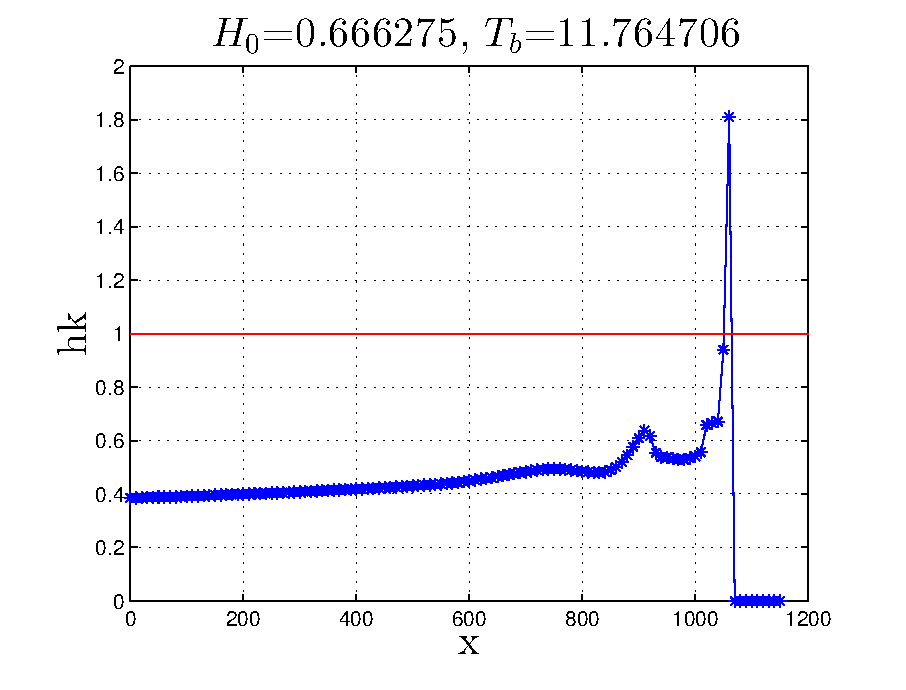
\includegraphics[width=\textwidth]{forward_plot/p1_2.eps}
%\caption{Example \eqref{ex1} Case I: $N=100$}
\label{Fighk_1}
\end{minipage}
\hspace{0.2cm}
\begin{minipage}[b]{0.47\linewidth}
\centering
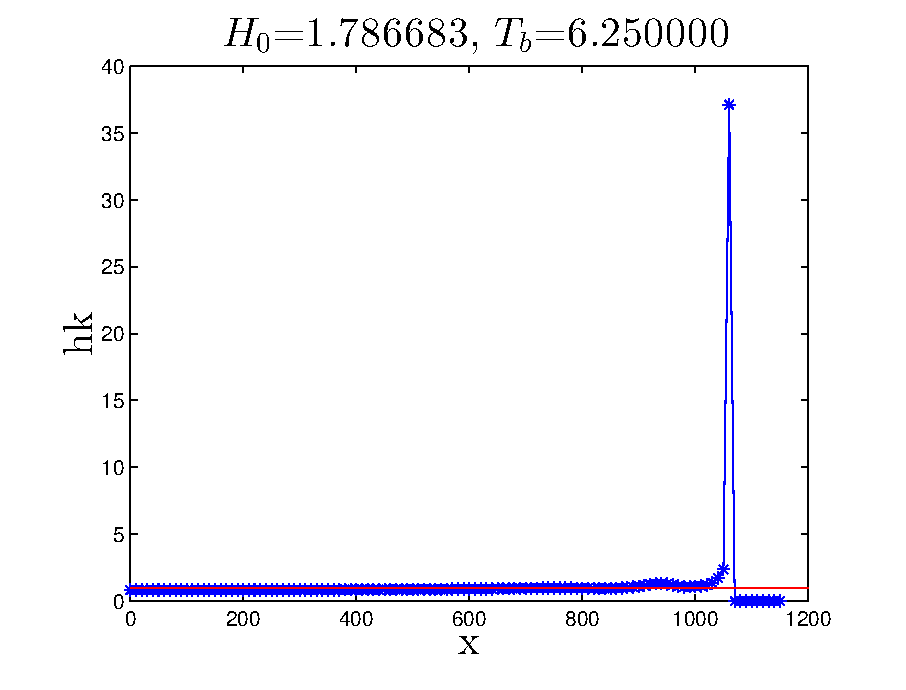
\includegraphics[width=\textwidth]{forward_plot/p2_2.eps}
%\caption{Example \eqref{ex1} Case I: $N=500$}
\label{Fighk_2}
\end{minipage}
\caption{Relative Depth varies with x direction}
\end{figure}
%%%%%%%%%%%%%%%%%%%%%%%%%%%%%%%%%%%%%%%%%%%%%%%%%%%%%%%%%%%%%%%%%%%%%%%%%%%%%%%%%%%%%%%%%%%%%%%%%%%%%%%%%%%%%%%%%%%%%%

%%%%%%%%%%%%%%%%%%%%%%%%%%%%%%%%%%%%%%%%%%%%%%%%%%%%%%%%%

\begin{figure}[h]
\begin{minipage}[b]{0.47\linewidth}
\centering
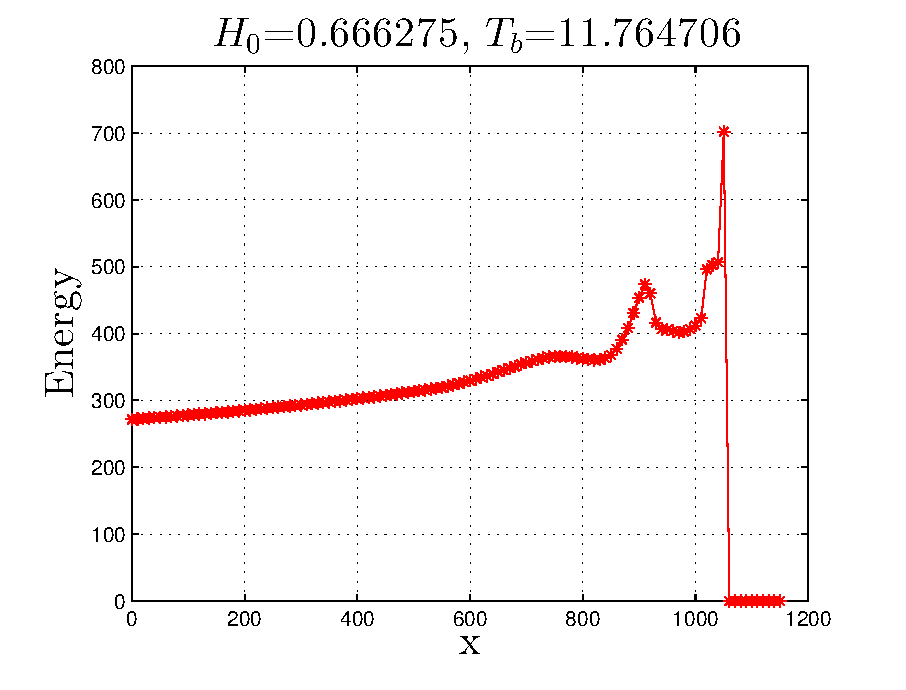
\includegraphics[width=\textwidth]{forward_plot/p1_3.eps}
%\caption{Example \eqref{ex1} Case I: $N=100$}
\label{Figenergy_1}
\end{minipage}
\hspace{0.2cm}
\begin{minipage}[b]{0.47\linewidth}
\centering
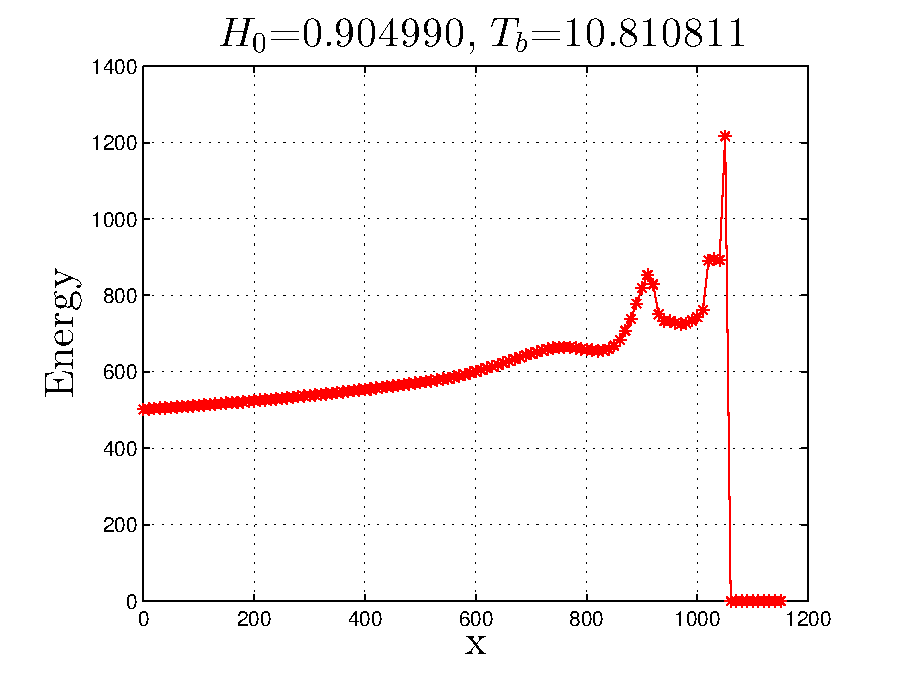
\includegraphics[width=\textwidth]{forward_plot/p2_3.eps}
%\caption{Example \eqref{ex1} Case I: $N=500$}
\label{Figenergy_2}
\end{minipage}
\caption{Wave Energy varies along x direction}
\end{figure}
%%%%%%%%%%%%%%%%%%%%%%%%%%%%%%%%%%%%%%%%%%%%%%%%%%%%%%%%%%%%%%%%%%%%%%%%%%%%%%%%%%%%%%%%%%%%%%%%%%%%%%%%%%%%%%%%%%%%%%

%%%%%%%%%%%%%%%%%%%%%%%%%%%%%%%%%%%%%%%%%%%%%%%%%%%%%%%%%

\begin{figure}[h]
\begin{minipage}[b]{0.47\linewidth}
\centering
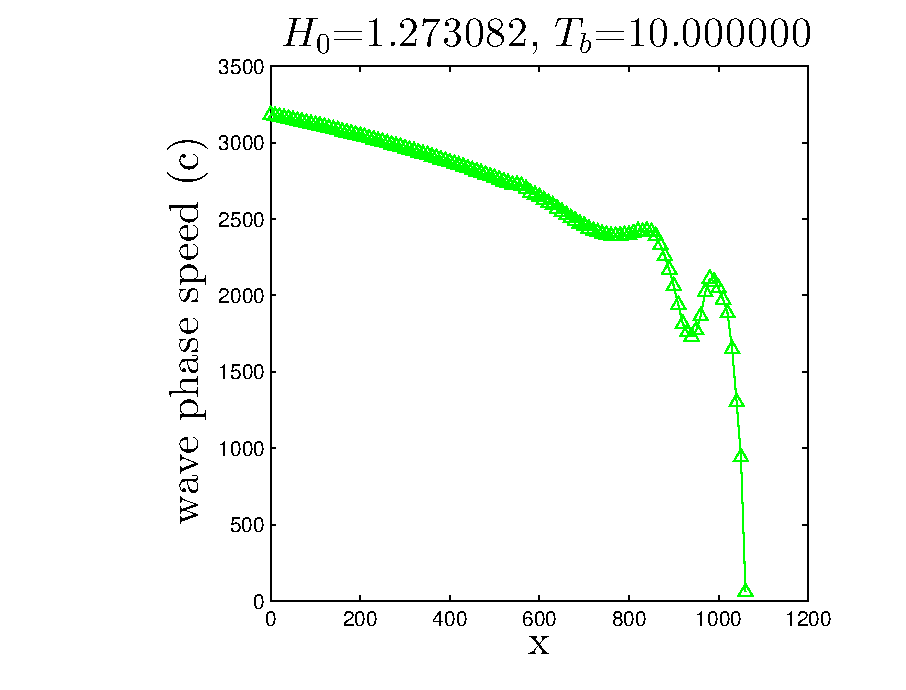
\includegraphics[width=\textwidth]{forward_plot/p1_4.eps}
%\caption{Example \eqref{ex1} Case I: $N=100$}
\label{Figc_1}
\end{minipage}
\hspace{0.2cm}
\begin{minipage}[b]{0.47\linewidth}
\centering
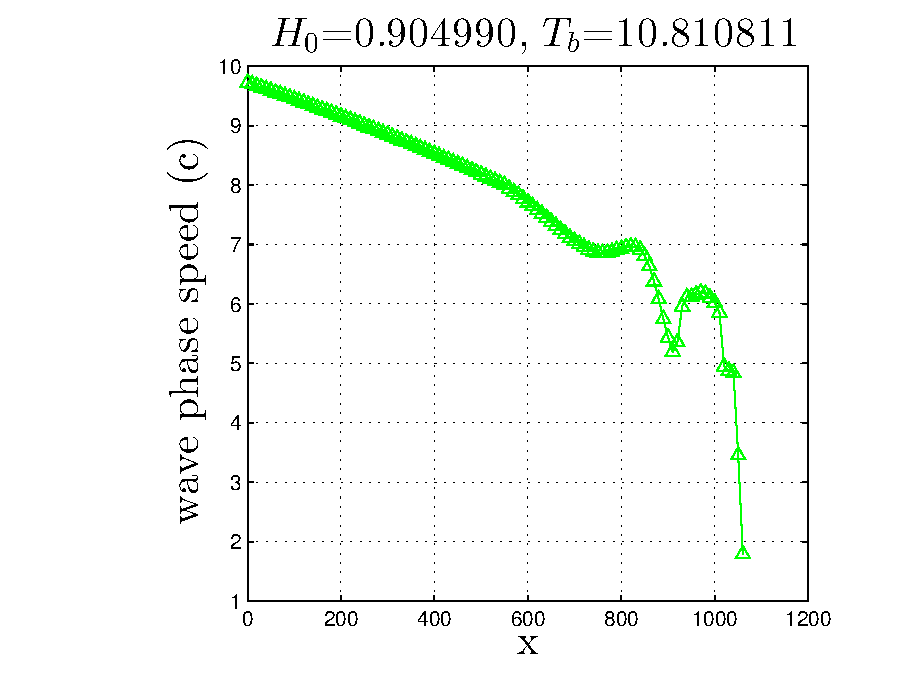
\includegraphics[width=\textwidth]{forward_plot/p2_4.eps}
%\caption{Example \eqref{ex1} Case I: $N=500$}
\label{Figc_2}
\end{minipage}
\caption{Wave Phase Speed (c) varies with x direction}
\end{figure}
%%%%%%%%%%%%%%%%%%%%%%%%%%%%%%%%%%%%%%%%%%%%%%%%%%%%%%%%%%%%%%%%%%%%%%%%%%%%%%%%%%%%%%%%%%%%%%%%%%%%%%%%%%%%%%%%%%%%%%%%%%%%%%%%%%%%%%%%%%%%%%%%%%%%%%%%%%%%%%%%%%%%%%%%%%%%%%%

\begin{figure}[h]
\begin{minipage}[b]{0.47\linewidth}
\centering
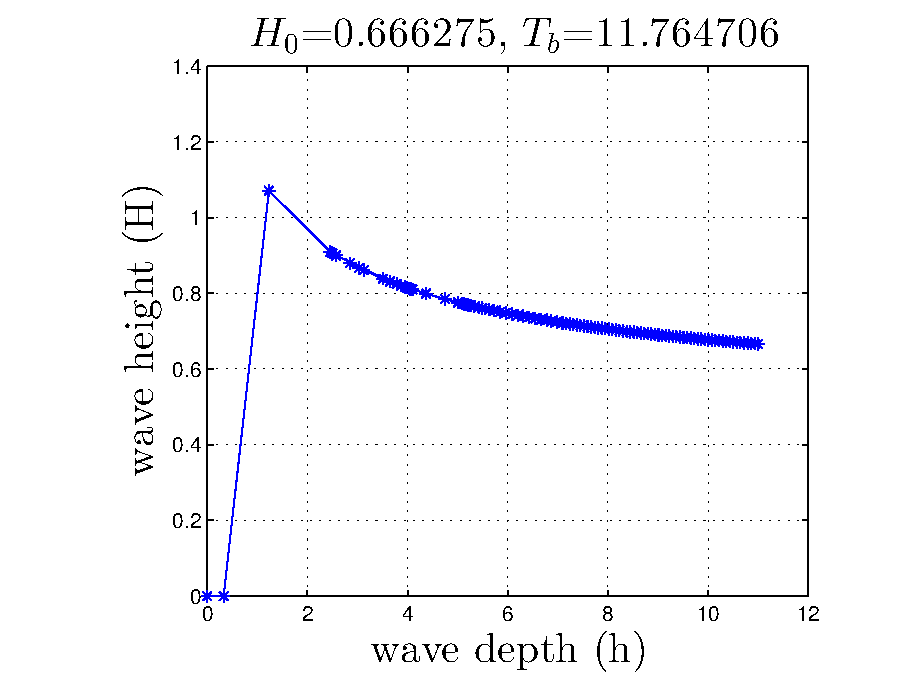
\includegraphics[width=\textwidth]{forward_plot/p1_5.eps}
%\caption{Example \eqref{ex1} Case I: $N=100$}
\label{FigH_1}
\end{minipage}
\hspace{0.2cm}
\begin{minipage}[b]{0.47\linewidth}
\centering
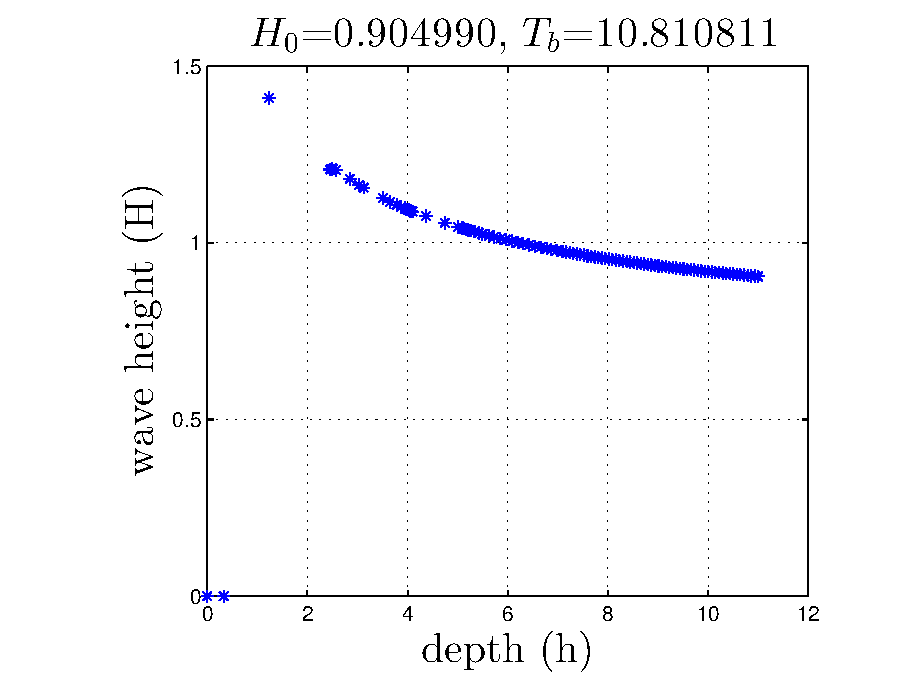
\includegraphics[width=\textwidth]{forward_plot/p2_5.eps}
%\caption{Example \eqref{ex1} Case I: $N=500$}
\label{FigH_2}
\end{minipage}
\caption{Wave Height(H) varies with Water Depth(h)}
\end{figure}
%%%%%%%%%%%%%%%%%%%%%%%%%%%%%%%%%%%%%%%%%%%%%%%%%%%%%%%%%%%%%%%%%%%%%%%%%%%%%%%%%%%%%%%%%%%%%%%%%%%%%%%%%%%%%%%%%%%%%%

%%%%%%%%%%%%%%%%%%%%%%%%%%%%%%%%%%%%%%%%%%%%%%%%%%%%%%%%%

\begin{figure}[h]
\begin{minipage}[b]{0.47\linewidth}
\centering
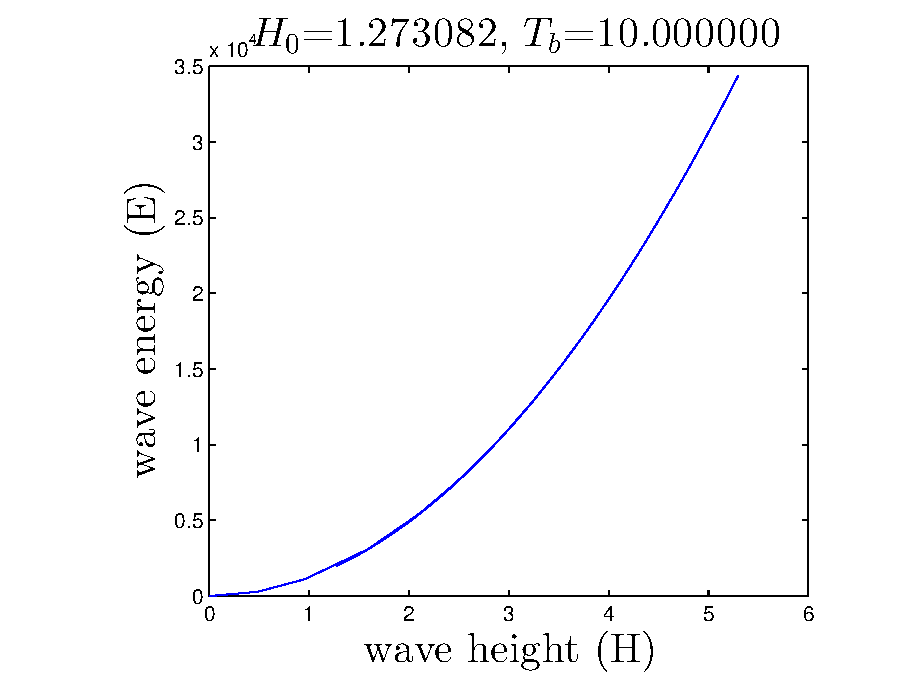
\includegraphics[width=\textwidth]{forward_plot/p1_6.eps}
%\caption{Example \eqref{ex1} Case I: $N=100$}
\label{FigE_1}
\end{minipage}
\hspace{0.4cm}
\begin{minipage}[b]{0.47\linewidth}
\centering
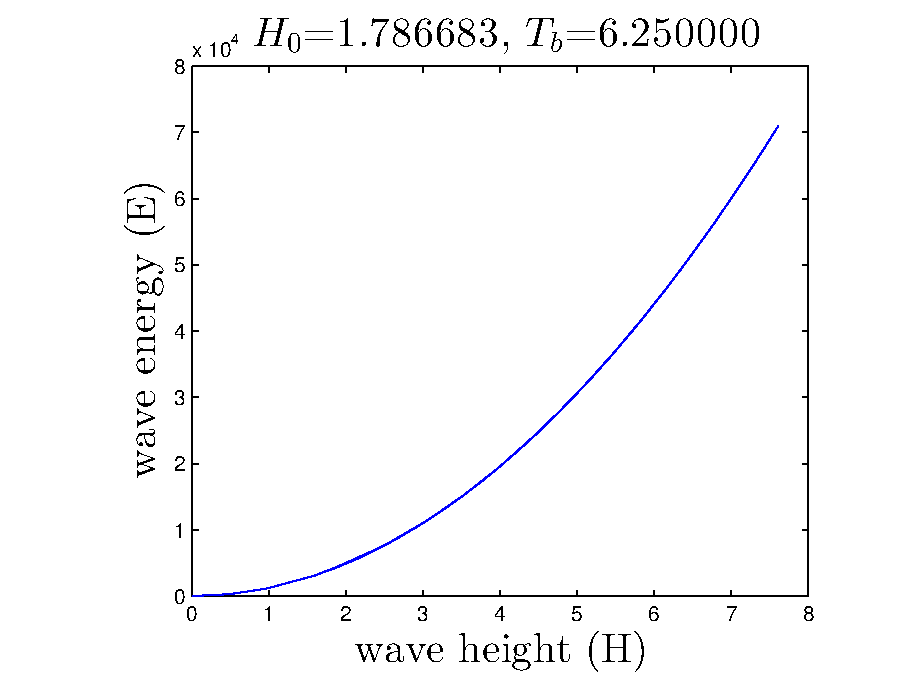
\includegraphics[width=\textwidth]{forward_plot/p2_6.eps}
%\caption{Example \eqref{ex1} Case I: $N=500$}
\label{FigE_2}
\end{minipage}
\caption{Wave Energy varies with Wave Height(H)}
\end{figure}
%%%%%%%%%%%%%%%%%%%%%%%%%%%%%%%%%%%%%%%%%%%%%%%%%%%%%%%%%%%%%%%%%%%%%%%%%%%%%%%%%%%%%%%%%%%%%%%%%%%%%%%%%%%%%%%%%%%%%%

\begin{figure}[h]
\begin{minipage}[b]{0.47\linewidth}
\centering
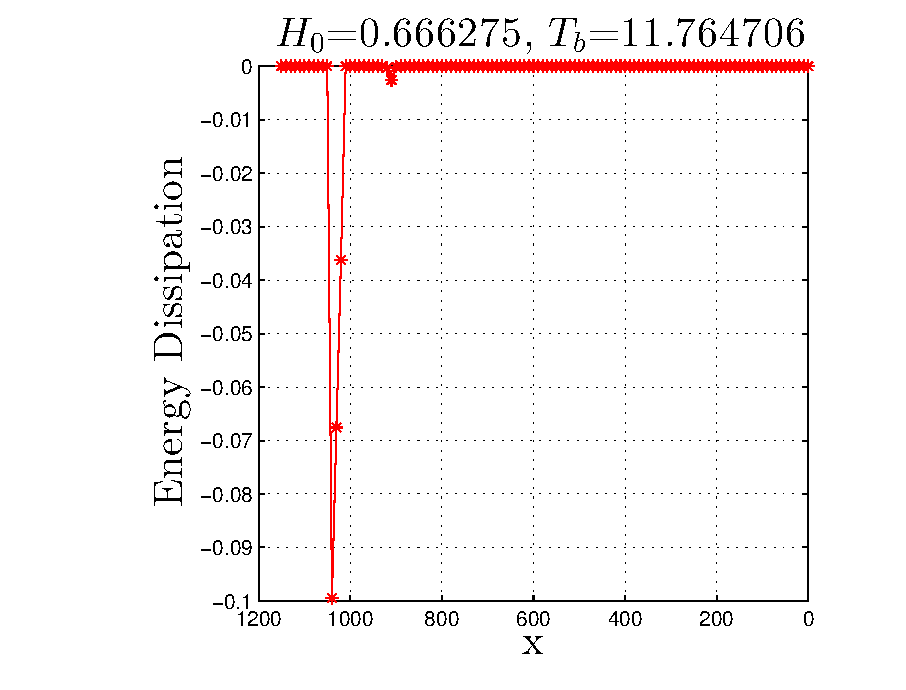
\includegraphics[width=\textwidth]{forward_plot/p1_7.eps}
%\caption{Example \eqref{ex1} Case I: $N=100$}
\label{FigE_1}
\end{minipage}
\hspace{0.4cm}
\begin{minipage}[b]{0.47\linewidth}
\centering
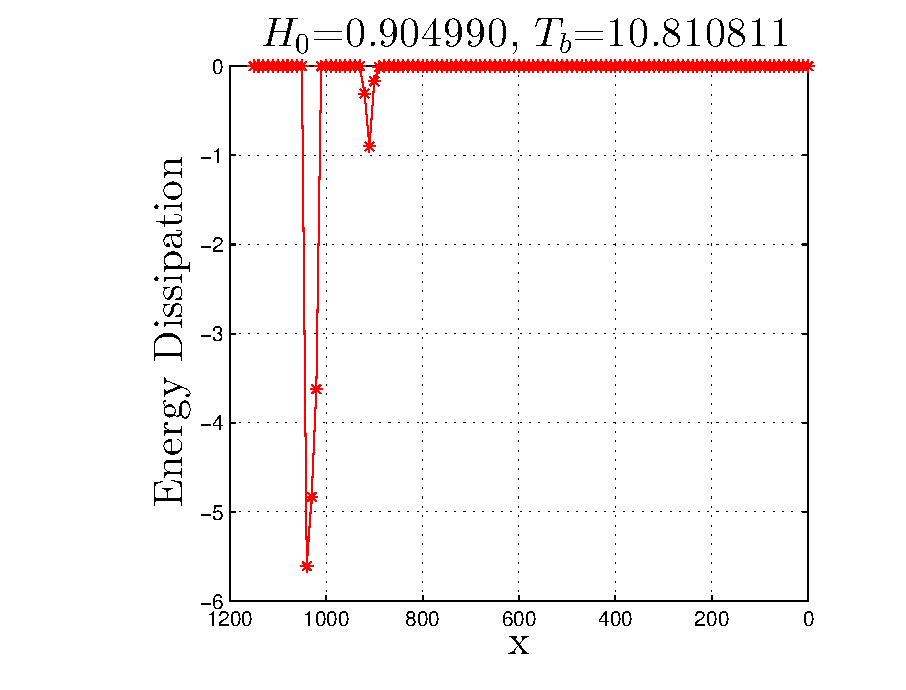
\includegraphics[width=\textwidth]{forward_plot/p2_7.eps}
%\caption{Example \eqref{ex1} Case I: $N=500$}
\label{FigE_2}
\end{minipage}
\caption{Wave Energy Dissipation varies along x-axis}
\end{figure}
